Conforme discutido na Seção~\ref{sec:related_works}, o MTLNet \cite{silva2025mtlnet} utiliza um único vetor $\mathbf{E}_{DGI} \in \mathbb{R}^{64}$ como entrada para ambas as tarefas, codificando informações espaciais e categóricas de forma conjunta por meio da topologia do grafo. Uma limitação dessa abordagem monolítica é que ela não incorpora coordenadas geográficas contínuas nem padrões temporais de visitação, fatores que, como demonstrado por trabalhos em codificação espacial \cite{wu2024torchspatial} e temporal \cite{kazemi2019time2vec}, carregam informações complementares às relações topológicas do grafo.

A decisão central de projeto deste trabalho é decompor a representação unimodal do DGI em três componentes independentes de 64 dimensões cada, treinados separadamente e integrados por concatenação: um \textit{encoder} espacial contínuo, um \textit{encoder} temporal (Time2Vec) e um \textit{encoder} categórico hierárquico (HGI). A hipótese subjacente é que uma representação desacoplada, com \textit{encoders} especializados treinados com funções de perda adequadas a cada dimensão da informação, produz representações mais expressivas do que uma representação unimodal que codifica todas as dimensões conjuntamente. Para avaliar essa hipótese e investigar o impacto da estratégia de codificação espacial, são comparados dois \textit{encoders} com pressupostos arquiteturais distintos: SIREN e Sphere2Vec-M.

A metodologia proposta é ilustrada na Figura~\ref{fig:arquitetura_arch}. A seguir são descritos o modelo MTLNet, o \textit{baseline} com DGI, a justificativa e o funcionamento de cada \textit{encoder} proposto, e a estratégia de integração dos \textit{embeddings}.


\begin{figure*}[htbp]
    \centering
    \makebox[\textwidth][c]{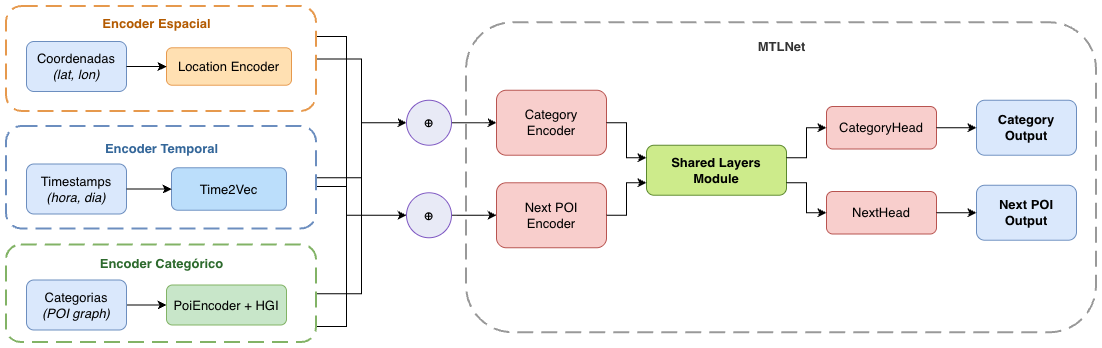
\includegraphics[width=1\textwidth]{imagens/arquitetura_modelo.png}}
    \caption{Arquitetura baseada no MTLNet \cite{silva2025mtlnet}. Os \textit{encoders} espacial, temporal e categórico são treinados de forma desacoplada e geram seus respectivos \textit{embeddings}, que são integrados como entrada do modelo e processados pelas camadas compartilhadas do modelo multitarefa (\textit{Shared Layers Module}) e pelas camadas específicas de cada tarefa, produzindo as saídas \textit{Category Output} e \textit{Next POI Output}.}
    \label{fig:arquitetura_arch}
\end{figure*}

O MTLNet \cite{silva2025mtlnet} é uma rede multitarefa construída sobre compartilhamento rígido de parâmetros (\textit{hard parameter sharing}) \cite{caruana1997multitask}, que processa simultaneamente as tarefas de classificação de categoria de POI e predição do próximo POI. A arquitetura utiliza \textit{encoders} específicos por tarefa implementados como MLPs com LayerNorm e Dropout, que projetam os \textit{embeddings} de entrada em um espaço latente compartilhado de dimensão $d_{\mathrm{shared}} = 256$. Em seguida, é aplicada a modulação FiLM (\textit{Feature-wise Linear Modulation}) \cite{perez2018film}, condicionada por um \textit{embedding} de identificador de tarefa $\mathbf{e}_{t}$, que gera parâmetros de escala $\gamma_{t}$ e deslocamento $\beta_{t}$ para modular as representações codificadas:

\begin{equation}
\mathrm{FiLM}(\mathbf{h}_{\mathrm{enc}}^{(t)} \,|\, \mathbf{e}_{t}) = \gamma_{t} \odot \mathbf{h}_{\mathrm{enc}}^{(t)} + \beta_{t}
\label{eq:film}
\end{equation}

As representações moduladas são processadas por quatro blocos residuais compartilhados com LayerNorm, LeakyReLU e Dropout, permitindo ao modelo aprender uma representação comum para ambas as tarefas \cite{baxter2000model}.

Na saída, cada tarefa possui uma \textit{head} especializada. O módulo de classificação de categoria utiliza um conjunto de três MLPs paralelas com profundidades variadas (2, 3 e 4 camadas), cujas saídas são concatenadas e projetadas para as 7 classes de POI. A \textit{head} de próximo POI emprega um \textit{Transformer encoder} com 8 \textit{heads} de atenção e 4 camadas, máscara causal para processamento autoregressivo, e \textit{pooling} ponderado por pesos de atenção aprendidos sobre os \textit{timesteps} da sequência de entrada. %(janela de tamanho $L_h = 9$).

O treinamento multitarefa utiliza o regularizador Nash-MTL \cite{nash}, que formula o balanceamento dos gradientes como um jogo cooperativo de barganha de Nash entre $K$ tarefas. Dados os gradientes de cada tarefa, o Nash-MTL busca a direção de atualização que maximiza o produto das utilidades de todas as tarefas, o que garante que a atualização seja benéfica para todas as tarefas simultaneamente, evitando a dominância de uma tarefa sobre a outra.


% \begin{equation}
% \Delta\boldsymbol{\theta}^{*} = \arg\max_{\Delta\boldsymbol{\theta} \in \mathcal{B}_\varepsilon}
% \sum_{k=1}^{K} \log\!\left(\mathbf{g}_k^{\top} \Delta\boldsymbol{\theta}\right)
% \quad\text{s.t. } \mathbf{g}_k^{\top} \Delta\boldsymbol{\theta} > 0,\;\forall k
% \label{eq:nash}
% \end{equation}

\subsection{Baseline: MTLNet com DGI}

O modelo \textit{baseline} corresponde ao MTLNet original proposto em \cite{silva2025mtlnet}, cuja arquitetura interna é mantida inalterada neste trabalho. Nesse modelo, cada POI é representado por um único \textit{embedding} monolítico $\mathbf{E}_{DGI} \in \mathbb{R}^{64}$, obtido via \textit{Deep Graph Infomax} (DGI) \cite{velickovic2019deep} sobre um grafo espacial construído por Triangulação de Delaunay e atributos categóricos dos nós, conforme descrito detalhadamente em \cite{silva2025mtlnet}. Assim, o DGI codifica conjuntamente relações espaciais e categóricas em um único vetor, sem incorporar componentes temporais explícitas. Em contraste, a abordagem proposta substitui essa representação monolítica pela concatenação de três \textit{encoders} especializados, totalizando 192 dimensões de entrada.


\subsection{Preparação dos Dados}

Para a tarefa de \textit{classificação de categoria de POI}, cada POI é representado pelo \textit{embedding} resultante da concatenação dos três componentes, $\mathbf{E}_{cat} = [\mathbf{E}_{HGI} \| \mathbf{E}_{loc} \| \mathbf{E}_{time}] \in \mathbb{R}^{192}$, formando pares $(\mathbf{E}_{cat}, c)$ onde $c$ é a categoria real do POI. No caso do \textit{baseline}, é utilizado diretamente $\mathbf{E}_{DGI} \in \mathbb{R}^{64}$.

Para a tarefa de \textit{predição do próximo POI}, os \textit{check-ins} são ordenados cronologicamente por usuário, e usuários com menos de cinco visitas são descartados. São extraídas janelas não sobrepostas de tamanho $L_h = 9$: os \textit{check-ins} $(p_1, \dots, p_9)$ formam o contexto, e $p_{\text{target}}$ é o próximo POI cuja categoria deve ser predita. Cada \textit{check-in} da janela é representado pelo \textit{embedding} correspondente, resultando em uma entrada de $9 \times 192 = 1728$ dimensões para o ST-MTLNet e $9 \times 64 = 576$ dimensões para o \textit{baseline}. Sequências mais curtas são preenchidas com \textit{padding} de vetores nulos.

\subsection{Encoder Espacial}

O modelo original MTLNet codifica informações espaciais de forma implícita por meio da topologia do grafo de Delaunay, sem utilizar diretamente as coordenadas geográficas como sinal de entrada. No entanto, como discutido na Seção~\ref{sec:related_works}, codificadores espaciais contínuos têm demonstrado eficácia em diversas tarefas geoespaciais \cite{wu2024torchspatial}, embora sua aplicação em modelos multitarefa de POIs permaneça pouco explorada. Este trabalho seleciona dois \textit{encoders} que representam paradigmas distintos de codificação espacial: o SIREN \cite{rußwurm2024geographiclocationencodingspherical}, que modela funções contínuas por ativações senoidais com frequências controláveis, e o Sphere2Vec-M \cite{mai2023sphere2vecgeneralpurposelocationrepresentation}, que opera diretamente em coordenadas esféricas preservando propriedades de distância geodésica. Essa diversidade permite avaliar como diferentes pressupostos geométricos e arquiteturais impactam o desempenho em tarefas de POI.

Todos os \textit{encoders} produzem $\mathbf{E}_{loc} \in \mathbb{R}^{64}$ e são 
treinados com a mesma função de perda contrastiva binária baseada na distância geográfica entre pares de coordenadas:
\begin{equation}
\mathcal{L}_{\text{loc}}(i,j)
=
- \left[
y_{ij}\,\log \sigma\!\left(\frac{\text{sim}(z_i,z_j)}{\tau}\right)
+
(1-y_{ij})
\log \left(1 - \sigma\!\left(\frac{\text{sim}(z_i,z_j)}{\tau}\right)\right)
\right]
\end{equation}

na qual $\sigma$ denota a função sigmoide, $\text{sim}(\cdot,\cdot)$ é a similaridade de cosseno, e $y_{ij} \in \{0,1\}$ indica se o par é positivo ($\Delta d_{ij} \leq 10$ km) ou negativo ($\Delta d_{ij} \geq 70$ km), com temperatura $\tau = 0{,}15$. A utilização da mesma função de perda para os dois \textit{encoders} espaciais permite uma comparação controlada, isolando o efeito da arquitetura de codificação.

% \subsubsection{Space2Vec-grid}

% O Space2Vec-grid proposto por Mai et al. \cite{mai2020multiscalerepresentationlearningspatial} realiza a modelagem espacial a partir das coordenadas contínuas de latitude e longitude dos \textit{check-ins} e pode ser definido em duas camadas principais:

% \begin{description}
%     \item[\textbf{Codificador Posicional Senoidal (\textit{Position Encoder}):}]
%     As coordenadas ($\lambda, \phi$) dos \textit{check-ins} são transformadas em um vetor de alta dimensão por meio de funções senoidais e cossenos com frequências logaritmicamente espaçadas.

%     \item[\textbf{Rede Neural \textit{Feed-Forward} (FFN):}]
%     O vetor de codificação posicional é processado por uma FFN de múltiplas camadas com \textit{skip connection} e LayerNorm, que projeta a representação no \textit{embedding} final $\mathbf{E}_{loc} \in \mathbb{R}^{64}$.
% \end{description}

\subsubsection{SIREN}

O modelo SIREN (\textit{Sinusoidal Representation Networks}) \cite{rußwurm2024geographiclocationencodingspherical} modela uma função contínua $f_\theta : \mathbb{R}^2 \rightarrow \mathbb{R}^{64}$ que mapeia diretamente coordenadas geográficas normalizadas em um \textit{embedding} vetorial. Cada camada da rede utiliza ativações senoidais com frequências controláveis, permitindo representar sinais de alta frequência em dados espaciais. A saída é o \textit{embedding} $\mathbf{E}_{loc} \in \mathbb{R}^{64}$.

\subsubsection{Sphere2Vec-M}

O Sphere2Vec-M \cite{mai2023sphere2vecgeneralpurposelocationrepresentation} é um codificador multi-escala formulado para operar diretamente em coordenadas esféricas ($\lambda$, $\phi$), gerando representações que preservem propriedades de distância na superfície da esfera. É utilizada a variante \textit{sphereM}, na qual são empregadas $S=16$ escalas multi-resolução com fatores geometricamente espaçados entre 10 km e 10.000 km. Termos de interação entre $\lambda$ e $\phi$ são construídos mantendo uma das componentes no maior nível de escala, permitindo controlar a resolução angular de latitude e longitude de forma independente. O vetor resultante é projetado por uma MLP para produzir $\mathbf{E}_{loc} \in \mathbb{R}^{64}$.

\subsection{Encoder Temporal}

Padrões de mobilidade humana apresentam regularidades cíclicas, como horários de refeição e deslocamentos semanais, que carregam informações discriminativas sobre a natureza funcional dos POIs visitados \cite{sun2020go}. No entanto, o modelo original MTLNet não incorpora representações temporais explícitas para capturar essas informações. 

Para preencher essa lacuna, é utilizado o Time2Vec \cite{kazemi2019time2vec}, uma representação temporal genérica e desacoplada capaz de capturar padrões periódicos e não periódicos sem necessidade de engenharia manual de \textit{features}. A arquitetura combina termos lineares e periódicos para mapear os valores temporais de cada \textit{check-in} (hora do dia e dia da semana, de forma acoplada) em um vetor de \textit{embedding}. Para um \textit{embedding} de dimensão $D$, a função é definida como:

\begin{equation}
\mathbf{f}(\tau)[i] = \begin{cases} \omega_0 \tau + \phi_0 & \text{se } i=0 \\ \sin(\omega_i \tau + \phi_i) & \text{se } 1 \leq i \leq D-1 \end{cases}
\label{eq:time2vec}
\end{equation}

na qual $\omega_i$ e $\phi_i$ são parâmetros treináveis (pesos e \textit{bias}) que capturam a periodicidade dos padrões temporais de visitação. O termo linear ($i=0$) captura tendências temporais globais, enquanto os termos senoidais modelam padrões cíclicos em diferentes frequências.

O modelo é treinado usando os valores temporais discretos (hora do dia e dia da semana) de forma acoplada para cada \textit{check-in}, com a mesma formulação contrastiva binária empregada no encoder espacial, sendo denominada $\mathcal{L}_{tempo}$. A saída final é o \textit{embedding} $\mathbf{E}_{time} \in \mathbb{R}^{64}$, que representa o \textit{timestamp} de cada \textit{check-in}.

\subsection{Encoder Categórico}

O DGI utilizado no modelo original codifica informações categóricas por meio de uma matriz \textit{one-hot} de 7 classes processada pela estrutura do grafo, sem capturar explicitamente relações hierárquicas ou regionais entre categorias de POIs. Para enriquecer essa dimensão, a geração de \textit{embeddings} categóricos é realizada em duas fases complementares. O POI Encoder aprende representações vetoriais que capturam coocorrências entre categorias a partir de caminhadas aleatórias no grafo espacial, e o modelo HGI \cite{huang2023learning} incorpora informações hierárquicas em múltiplos níveis (POI, região e cidade), produzindo representações que refletem tanto o contexto local quanto o regional.

\subsubsection{POI Encoder}

O POI Encoder é treinado de forma independente para gerar o \textit{embedding} de categoria $\mathbf{E}_{\text{POI\_categoria}} \in \mathbb{R}^{64}$. Os POIs são organizados em um grafo espacial construído por Triangulação de Delaunay sobre as coordenadas geográficas, com arestas ponderadas por decaimento logarítmico da distância Haversine e penalização para conexões entre condados (GEOIDs) distintos.

Sobre esse grafo são executadas caminhadas aleatórias (\textit{random walks}) seguindo a metodologia do Node2Vec \cite{grover2016node2vec}. Cada caminhada é convertida em uma sequência de categorias secundárias (\textit{fclass}), resultando em coocorrências locais e globais entre categorias. O modelo aprende os \textit{embeddings} utilizando a estratégia \textit{skip-gram} com \textit{negative sampling} \cite{church2017word2vec}:

\[
\mathcal{L}_{\text{SGNS}}(i,j)
=
-\log \sigma\!\left(\mathbf{e}_j^\top \mathbf{e}_i\right)
-
\sum_{k=1}^{K}
\log \sigma\!\left(-\mathbf{e}_{n_k}^\top \mathbf{e}_i\right),
\]

na qual $\mathbf{e}_i$ é o \textit{embedding} da classe alvo, $\mathbf{e}_j$ o \textit{embedding} positivo de contexto, e $\mathbf{e}_{n_k}$ representam as amostras negativas. A implementação incorpora um termo de regularização hierárquica \cite{belkin2003laplacian} entre categoria e \textit{fclass}: $\mathcal{L}_{\text{hier}} = \sum_{(c,s) \in \mathcal{H}} \left\| \mathbf{e}_s - \mathbf{e}_c \right\|_2^2$, na qual $\mathcal{H}$ contém os pares (categoria, \textit{fclass}). A perda total é $\mathcal{L} = \mathcal{L}_{\text{SGNS}} + \lambda_{\text{hier}} \, \mathcal{L}_{\text{hier}}$. Ao final, o \textit{embedding} resultante é gerado por categoria e remapeado para cada POI.

\subsubsection{Hierarchical Graph Infomax (HGI)}

Após a geração dos \textit{embeddings} $\mathbf{E}_{\text{POI\_categoria}}$, eles são utilizados como entrada para o modelo Hierarchical Graph Infomax (HGI) \cite{huang2023learning}, que enriquece a representação incorporando informações geográficas regionais. O modelo otimiza a informação mútua em dois níveis hierárquicos (POI-região e região-cidade):

\[
\mathcal{L}
=
\alpha\,\mathcal{L}_{\text{POI--região}}
+
(1-\alpha)\,\mathcal{L}_{\text{região--cidade}},
\]

na qual $\alpha = 0{,}5$ controla o equilíbrio entre os níveis hierárquicos. Ambas as perdas utilizam amostragem negativa estrutural para reforçar a separabilidade entre regiões e entre POIs. A saída são os \textit{embeddings} enriquecidos $\mathbf{E}_{\text{HGI}} \in \mathbb{R}^{64}$, que capturam relações categóricas tanto locais quanto regionais.



\subsection{Integração dos Embeddings}

Os três componentes de representação são treinados de forma independente e concatenados para formar a entrada de ambas as tarefas do MTLNet:

\begin{equation}
\mathbf{E}_{input} = [\mathbf{E}_{HGI} \| \mathbf{E}_{loc} \| \mathbf{E}_{time}] \in \mathbb{R}^{192}
\label{eq:concat}
\end{equation}

A escolha da concatenação como estratégia de integração preserva a informação individual de cada componente sem impor interações prematuras entre as representações, delegando ao MTLNet a tarefa de aprender como combinar essas dimensões por meio de suas camadas compartilhadas e da modulação FiLM. A dimensionalidade de entrada do ST-MTLNet ($\mathbb{R}^{192}$) é superior à do \textit{baseline} ($\mathbb{R}^{64}$), uma consequência natural da decomposição em três componentes. No entanto, a arquitetura do MTLNet projeta qualquer entrada para o mesmo espaço latente compartilhado de dimensão $d_{\mathrm{shared}} = 256$ por meio dos \textit{encoders} específicos por tarefa, de modo que a capacidade das camadas compartilhadas e das cabeças de tarefa permanece inalterada.

São avaliadas duas variantes do modelo proposto, denominadas ST-MTLNet (\textit{Spatial-Temporal MTLNet}), cada uma utilizando um \textit{encoder} espacial diferente. O \textit{baseline} MTLNet \cite{silva2025mtlnet} utiliza somente o \textit{embedding} monolítico $\mathbf{E}_{DGI} \in \mathbb{R}^{64}$ como entrada para ambas as tarefas. As variantes propostas substituem essa representação pela concatenação dos \textit{embeddings} desacoplados, mantendo fixos os \textit{encoders} temporal (Time2Vec) e categórico (HGI) e variando o \textit{encoder} espacial entre SIREN e Sphere2Vec-M.

Todos os modelos compartilham os mesmos hiperparâmetros da arquitetura MTLNet, diferindo apenas nos \textit{embeddings} de entrada. Essa configuração permite isolar o efeito da estratégia de representação sobre o desempenho, avaliando tanto o ganho da abordagem modular em relação ao \textit{baseline} monolítico quanto o impacto da escolha do \textit{encoder} espacial.